% 12_alternatives.tex -- Part 12, alternative explanations and uncertainty. Sources: research_monograph/chapters/
% M13_alternatives_uncertainty.tex (tab:mono-alt-tc, sec:mono-alt-6p3, tab:mono-alt-budget, keyresult),
% M06_defect_theory.tex (sec:mono-defect-hydrogenic, sec:mono-defect-compensation, keyresult), 09_mechanisms_rev.tex
% (6.3 nm hypothesis study A1-A5, rigid/shape decomposition), M12_multiscale.tex (tab:mono-ms-budget, recommendations),
% M05_confinement_theory.tex (extrapolation of the laws), M04_dft_theory.tex (PBE gap), M15_conclusions.tex (required
% measurements and calculations); appendices/MG_corrections.tex (V1 SCF noise, V6 dielectric bound, V8 compensation,
% V10 extrapolation); evidence/FACT_REGISTRY.tsv (FACT-002, 025, 030, 080, 101, 102); evidence/CLAIM_SOURCE_MAP.tsv
% (M006, C014, C016, C018, C026, C028, C029, C037); evidence/derived/defect_estimates.json, multiscale_budget.json.
% Figure 12_binding.pdf: tools/fig_12_donor_binding.py (hydrogenic formulas of M06; checked against FACT-080).
% No amorphous electronic quantity; no ATLAS result from stage S2 on (S1-05 is quoted as in M08/M12).
% Note: frame bodies start with a command, never with a brace group (beamer would read a subtitle).
\partslide{Part 12}{Alternative explanations and uncertainty}

% denser slides: footnotesize bullets, local to the frame in which it is called
\providecommand{\twelvedense}{\setbeamerfont{itemize/enumerate body}{size=\footnotesize}%
  \setbeamerfont{itemize/enumerate subbody}{size=\footnotesize}}
\providecommand{\twelveTop}{\vspace{-4mm}}
\providecommand{\twelveData}{Data: Prof.\ M.-H.\ Lee's group, NTU; one device per thickness}
% re-use the mark of a footnote already placed on the same slide (same work cited twice)
\providecommand{\twelveSee}[1]{\hbox{\,{\usebeamercolor[fg]{footnote mark}\scriptsize[#1]}}}

% ---------------------------------------------------------------------------------------------------------------------
\begin{frame}[t]{Five explanations of the thickness step remain open}
  \twelveTop\twelvedense
  \footnotesize
  Observed, one device per film. From 2.0 to 6.3\,nm: $\Delta\Vthcc = -0.018$\,V, peak $\mu_{\mathrm{FE}}$\,$\times0.9$,
  $I_{\mathrm{on}}$\,$\times0.79$. From 6.3 to 13.2\,nm: $-0.561$\,V, $\times4.6$, $\times7.6$. The 31.8\,nm device
  does not switch off \lab{observed}.\par
  \vspace{0.6mm}
  % plain tabular (not tabularx): tabularx typesets its body several times and would duplicate the footnote
  \begingroup\scriptsize
  \setlength{\tabcolsep}{4.5pt}
  \renewcommand{\arraystretch}{1.12}
  \begin{tabular}{@{}>{\raggedright\arraybackslash}p{2.95cm}>{\raggedright\arraybackslash}p{7.05cm}>{\raggedright\arraybackslash}p{3.3cm}@{}}
    \toprule
    Explanation & For and against & Discriminating test \\
    \midrule
    Back-surface depletion by an air-side charge $N_s$
      & $W_{\mathrm{dep}} = N_s/N_D = 0.4$--40\,nm ($N_D = 2.5\times10^{17}$--$2.7\times10^{18}$\cmcu,
        $N_s = 10^{11}$--$10^{12}$\cmsq): a 6--13\,nm crossover without W \lab{derived}
      & capping, or vacuum against air, must move the crossover \\
    Donor density rising with thickness
      & the device fit needs exactly this, $N_{D,\mathrm{eff}} \propto 1 + (t/20\,\mathrm{nm})^4$, but it is not
        identifiable \lab{fitted}
      & depth-resolved composition \\
    Structural change (grains, crystallinity)
      & smaller grains for IWO than for \InO{} at comparable thickness\sref[p.~2]{Januar2026}; not quantified for these
        devices
      & GIXRD and TEM on the same films \\
    Donor deactivation by confinement
      & binding several times the bulk 25\,meV for $t < a_B^* = 2.7$\,nm; W-independent; not computed \lab{theory}
      & Hall density against thickness, \InO{} and IWO \\
    Smooth law plus device spread
      & with one device per film, indistinguishable from the rows above
      & $\ge$5--10 devices per thickness \\
    \bottomrule
  \end{tabular}\par\endgroup
  \src{Debye length 2.4--7.8\,nm; V1 back-charge runs 0030, 0035 did not settle depletion. W-specific loss of extended
    carriers (H-N): \textsc{unresolved} by construction (Part 11). Proposed series: about 1\,nm steps from 3 to 15\,nm
    at 0, 2 and 4\,at.\,\% W, several devices each. \twelveData\twelveSee{1}; C026, C029.}
  \takeaway{A dense thickness series, capped and uncapped, would decide between them.}
\end{frame}

% ---------------------------------------------------------------------------------------------------------------------
\begin{frame}[t]{Six tested mechanisms fail at 6.3\,nm; spread is untested}
  \twelveTop\twelvedense
  \begingroup\scriptsize
  \setlength{\tabcolsep}{4.5pt}
  \renewcommand{\arraystretch}{1.1}
  \begin{tabularx}{\textwidth}{@{}>{\raggedright\arraybackslash}p{3.7cm}>{\raggedright\arraybackslash}X>{\raggedright\arraybackslash}p{2.75cm}@{}}
    \toprule
    Candidate (V1 ATLAS run) & Result against the required $+0.294$\,V (run 0014) & Verdict \\
    \midrule
    Thickness error, $t = 5.3$\,nm (0031) & $+0.036$\,V (12\,\%); via $\dEc$ alone needs $t \approx 2.1$\,nm (67\,\% error)
      & rejected \\
    Fewer donors (0032) & $+0.030$\,V, a factor of ten short & rejected \\
    Back-surface charge (0030) & matches $\Vthcc$, but the swing is off by $-64.1$\,mV/dec & rejected as sole cause \\
    Front $D_{\mathrm{it}}\times5$ (0033) & $+0.051$\,V; the full miss needs $\times$23--24, at 6.3\,nm only &
      rejected at plausible $D_{\mathrm{it}}$ \\
    Combination (0035) & 0.215 of 0.294\,V (73\,\%); swing off by $-45.9$\,mV/dec & rejected \\
    Uniform donors (6.3--13.2\,nm)$^{\ast}$ & $2.2\times10^{18}$\cmcu: $-0.25$\,V at 2.0--6.3\,nm (measured $-0.018$\,V)
      & rejected \\
    Film-specific front charge (0015) & $Q_f = 8.7\times10^{10}$ instead of $1.73\times10^{12}$\cmsq{} fits & a
      calibration \lab{fitted} \\
    \midrule
    Spread, batch, sweep history & not testable with one device per film & open \\
    Non-monotonic electrostatics (H3) & prior low (C028) & open \\
    \bottomrule
  \end{tabularx}\par\endgroup
  \src{Rejections are model-conditional (V1 calibration) \lab{computed}; $^{\ast}$1-D surrogate, not ATLAS.
    \twelveData\sref{Januar2026}.}
  \vspace{-0.6mm}
  \begin{itemize}\setlength{\itemsep}{0pt}
    \item The miss is a rigid 0.294\,V (within 3\,mV from $10^{-11}$ to $10^{-9}$\,A/\textmu m) plus a shape part,
      $+0.16$/$+0.19$\,V at $10^{-7}$/$2\times10^{-7}$\,A/\textmu m, independent of the $\dEc$ law and of $Q_f$
      \lab{computed}.
    \item Decisive: $\ge$10 devices at 2, 4, 6.3, 9 and 13\,nm from one run; H3 is falsified if 6.3\,nm lies on a
      smooth trend.
  \end{itemize}
  \takeaway{For now, spread or a fabrication difference explains 6.3\,nm most economically.}
\end{frame}

% ---------------------------------------------------------------------------------------------------------------------
\begin{frame}[t]{Confinement can deactivate shallow donors, independent of W}
  \twelveTop\twelvedense
  \begin{columns}[T,onlytextwidth]
    \begin{column}{0.635\textwidth}
      \footnotesize
      Hydrogenic donor, $m^* = 0.208\,m_0$, $\varepsilon_s = 10.55$\sref[p.~225102-1]{Stokey2021} \lab{derived}:\par
      \vspace{0.6mm}
      \centerline{$E_D = \dfrac{m^*/m_0}{\varepsilon_s^2}\,\mathrm{Ry} = 25.4\,\mathrm{meV}, \qquad
        a_B^* = \dfrac{\varepsilon_s}{m^*/m_0}\,a_0 = 2.68\,\mathrm{nm}$}
      \vspace{0.4mm}
      {\scriptsize Ry = 13.606\,eV, $a_0 = 0.0529$\,nm; Mott: $n_c^{1/3}a_B^* \approx 0.26$,
        $n_c = 9.1\times10^{17}$\cmcu.\par}
      \vspace{-0.2mm}
      \begin{itemize}\setlength{\itemsep}{0pt}
        \item $t = 2$\,nm $\approx 0.75\,a_B^*$: quantum confinement roughly doubles $E_D$; strict 2-D limit $4\times$,
          0.10\,eV\sref{Bastard1981b} \lab{theory}.
        \item Beyond $r_0 = \varepsilon_s t/(\varepsilon_1+\varepsilon_2) \approx 2.1$\,nm the surroundings
          screen\sref{Cudazzo2011}: 0.45\,eV for \AlO/air, little gain on the \HfO-backed stack (V6). Such deactivation
          is known in Si nanowires\srefs{Diarra2007,Bjork2009}.
        \item 2\,\% W fully active: $6\times10^{20}$--$1.8\times10^{21}$\cmcu; fit: $2.5\times10^{17}$--$1.8\times
          10^{18}$\cmcu{} (C016): compensation or inactive donors\sref{Lany2007}, an argument of scale
          \lab{inferred}.
      \end{itemize}
    \end{column}
    \begin{column}{0.34\textwidth}
      \centering
      \vspace{-1mm}
      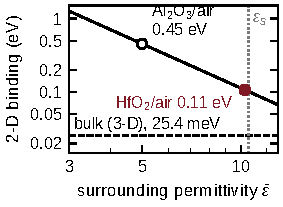
\includegraphics[width=\linewidth]{12_binding}\par
      \raggedright
      \src{Strict 2-D bound $4\,\mathrm{Ry}\,(m^*/m_0)/\bar\varepsilon^{\,2}$, $\bar\varepsilon = (\varepsilon_1 +
        \varepsilon_2)/2$ (\AlO{} $\approx 9$, \HfO{} 19.57, air 1). Grey: device stack; dotted: $\varepsilon_s$;
        dashed: bulk $E_D$. \lab{theory}; FACT-080.}
    \end{column}
  \end{columns}
  \takeaway{A W-independent route to fewer active donors in thin films; not computed here.}
\end{frame}

% ---------------------------------------------------------------------------------------------------------------------
\begin{frame}[t]{The largest uncertainties are not numerical}
  \twelveTop
  % plain tabular (not tabularx): tabularx typesets its body several times and would duplicate the footnote
  \begingroup\scriptsize
  \setlength{\tabcolsep}{4.2pt}
  \renewcommand{\arraystretch}{1.12}
  \begin{tabular}{@{}>{\raggedright\arraybackslash}p{2.75cm}>{\raggedright\arraybackslash}p{5.3cm}>{\raggedright\arraybackslash}p{1.25cm}>{\raggedright\arraybackslash}p{3.75cm}@{}}
    \toprule
    Source & Size or effect & Quantified & How it would be reduced \\
    \midrule
    One device per thickness & spread unknown; it enters every film-to-film difference (C026) & no &
      $\ge$10 devices per thickness, one run, dual sweeps \\
    Thickness values and definition & nominal values, method unknown; H--H or nominal: $\pm0.2$\,nm
      $\approx\pm40$\,mV in $\Vthcc$ at 2\,nm & partly & XRR and TEM on the same films; state the definition \\
    Crystalline PBE inputs for amorphous films & (001) slabs, OH termination; amorphous shift sealed (H-K); ML force
      check failed (C037) & partly & release of H-K; re-registered series, $\ge$2 seeds per endpoint \\
    Density-of-states convention at 2\,nm & quasi-2-D against 3-D $N_c$: 142\,mV in $\Vthcc$ (S1-05), a third to
      two thirds of a 6.3\,nm miss & yes & state it with every fitted charge \\
    PBE gap and functional & 0.89\,eV against 2.7--2.9\,eV measured\srefs{Walsh2008,Irmscher2014}: only differences
      used; HSE06/PBE ratio 1.06--1.11 (1\,nm): $+16$ to $+29$\,mV at 2\,nm
      & partly & optical gap against thickness; hybrid-functional W cell \\
    Extrapolated laws & computed to 1.96\,nm, used 3--7 times beyond; $\dEc(6.3\,\mathrm{nm}) = 0.050$--0.075\,eV over
      fit options & partly & optical gap, C--V flat band against thickness \\
    \bottomrule
  \end{tabular}\par\endgroup
  \src{Effects on $\Vthcc$ \lab{derived} (laws, audit A13); S1-05 \lab{computed} (ATLAS, seen before register revision
    2). Not limiting: registered DFT convergence, SCF force noise $\approx6\times10^{-5}$\,Ry/bohr per component, TCAD
    numerics $\approx0.7$\,\%. Non-identifiable threshold parameters (C018): Part 4.}
  \takeaway{Device statistics, thickness metrology and the $N_c$ convention dominate.}
\end{frame}
